\scanpage{96}
by conjecturing that these \inserted{necessary} conditions are sufficiently draconian \deleted{to} (even without entering into the consideration of the $\Theta^\nu$) to ensure that $\Theta$ does indeed come from a $u\in\Gamma$, \deleted{when} when $X$ is (say) an \uline{anabelian algebraic curve}, with a finitely generated extension of $\mathbb{Q}$.
\margin{I do not quite see whether condition a), without b), should be sufficient to ensure that $\Theta$ comes from $\Gamma$. And then, \unsure{in} all these \unsure{others}, and for profinite groups...}
\margin{
\figure{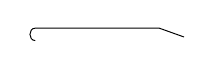
\begin{tikzpicture}[x=.45cm,y=.45cm]
\draw[line width=.35pt] (0,-.35) .. controls (-.2,-.35) and (-.2,0) .. (0,0) -- (3.5,0) -- (4.2,-.25);
\end{tikzpicture}}
\deleted{one \unsure{can}} not obvious that the anabelian hypothesis is required --- to be examined! (\unsure{Is not} \illegible{?} for $\mathbb{G}_m$, or an elliptic curve). The variation : $X/K$ of dimension $1$ also seems inessential to me. In fact, it is false for $\mathbb{G}_m$
\figure{\begin{tikzpicture}[x=.45cm,y=.45cm]
\draw[line width=.35pt] (0,0) -- (4.2,0) -- (4.2,.35) -- (5.15,.35);
\end{tikzpicture}}
}
\figure{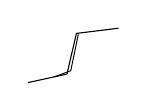
\begin{tikzpicture}[x=.6cm,y=.6cm]
\draw[line width=.4pt] (0,0) -- (.82,.18) -- (1.02,1.04) -- (1.91,1.15);
\draw[line width=.35pt] (.55,.12) -- (.9,.25) -- (1.06,1.02);
\end{tikzpicture}}
Of course, the question of the uniqueness of $u$ is not involved here --- when $K$ is an algebraic extension of $\mathbb{Q}$, one expects the \uline{uniqueness} of $u$. When $K$ is of transcendence degree $>0$, then in order to be able to expect uniqueness of $u$, one must at least suppose that the field of moduli of $X$ has $=$ transcendence degree, i.e. that $K$ is a \uline{finite} extension of this field of moduli. I would not be surprised if one had uniqueness in this case.
\margin{It must even be possible to prove this with what I know, \unsure{i.e.} via Белый. For uniqueness, of course, the anabelian condition is absolutely essential...}

I return to the question of the liftability of an \deleted{$\Theta$} endomorphism $\Theta$ of a connected groupoid $\mathcal{C}$ to a covering $\widetilde{\mathcal{C}}$, when $\Theta$ fixes a vertex
\margin{95}
